\documentclass{article}

% if you need to pass options to natbib, use, e.g.:
% \PassOptionsToPackage{numbers, compress}{natbib}
% before loading nips_2018

% ready for submission
\usepackage{nips_2018}

% to compile a preprint version, e.g., for submission to arXiv, add
% add the [preprint] option:
% \usepackage[preprint]{nips_2018}

% to compile a camera-ready version, add the [final] option, e.g.:
% \usepackage[final]{nips_2018}

% to avoid loading the natbib package, add option nonatbib:
% \usepackage[nonatbib]{nips_2018}

\usepackage[utf8]{inputenc} % allow utf-8 input
\usepackage[T1]{fontenc}    % use 8-bit T1 fonts
\usepackage{hyperref}       % hyperlinks
\usepackage{url}            % simple URL typesetting
\usepackage{booktabs}       % professional-quality tables
\usepackage{amsfonts}       % blackboard math symbols
\usepackage{nicefrac}       % compact symbols for 1/2, etc.
\usepackage{microtype}      % microtypography
\usepackage{stmaryrd}

\newcommand{\theHalgorithm}{\arabic{algorithm}}
\newcommand{\sem}[1]{\llbracket #1 \rrbracket}
\newcommand{\system}{\textsc{ECC}~}
\newcommand{\systemEnding}{\textsc{ECC}}
\newcommand{\lowerBound}{\mathscr{L}}
\newcommand{\code}[1]{{\footnotesize\texttt{#1}}}
\newcommand{\codechar}[1]{{\footnotesize{\texttt{"#1"}}}}

\usepackage{mathrsfs}
\usepackage{listings}
\usepackage{amsthm}

\usepackage{subfig} 
\usepackage{fancyvrb}


\usepackage{caption}
\usepackage{amssymb}
\usepackage{listings}
\usepackage{wrapfig}
\usepackage{tabularx}


\usepackage{verbatim}
 \usepackage{booktabs}
 % For algorithms
\usepackage{algorithm}
\usepackage{algorithmic}
\usepackage{tikz}
\usepackage{circuitikz}
\usetikzlibrary{fit,bayesnet}
\usepackage{dsfont}
\usepackage{amsmath}

\DeclareMathOperator*{\argmin}{arg\,min} % thin space, limits underneath in displays
\DeclareMathOperator*{\argmax}{arg\,max} % thin space, limits underneath in displays
 


% Packages hyperref and algorithmic misbehave sometimes.  We can fix
% this with the following command.

\newcommand{\Expect}{\mathds{E}} %{{\rm I\kern-.3em E}}
\newcommand{\indicator}{\mathds{1}} %{{\rm I\kern-.3em E}}
\newcommand{\expect}{\mathds{E}} %{{\rm I\kern-.3em E}}
\newcommand{\probability}{\mathds{P}} %{{\rm I\kern-.3em P}}

\title{Learning Libraries of Subroutines for Neurally--Guided Bayesian Program Learning}

% The \author macro works with any number of authors. There are two
% commands used to separate the names and addresses of multiple
% authors: \And and \AND.
%
% Using \And between authors leaves it to LaTeX to determine where to
% break the lines. Using \AND forces a line break at that point. So,
% if LaTeX puts 3 of 4 authors names on the first line, and the last
% on the second line, try using \AND instead of \And before the third
% author name.

\author{
  David S.~Hippocampus\thanks{Use footnote for providing further
    information about author (webpage, alternative
    address)---\emph{not} for acknowledging funding agencies.} \\
  Department of Computer Science\\
  Cranberry-Lemon University\\
  Pittsburgh, PA 15213 \\
  \texttt{hippo@cs.cranberry-lemon.edu} \\
  %% examples of more authors
  %% \And
  %% Coauthor \\
  %% Affiliation \\
  %% Address \\
  %% \texttt{email} \\
  %% \AND
  %% Coauthor \\
  %% Affiliation \\
  %% Address \\
  %% \texttt{email} \\
  %% \And
  %% Coauthor \\
  %% Affiliation \\
  %% Address \\
  %% \texttt{email} \\
  %% \And
  %% Coauthor \\
  %% Affiliation \\
  %% Address \\
  %% \texttt{email} \\
}

\begin{document}
% \nipsfinalcopy is no longer used

\maketitle

\begin{abstract}
  Successful approaches to program induction require a hand-engineered
  domain-specific language (DSL), constraining the space of allowed
  programs and imparting prior knowledge of the domain.  We contribute
  a program induction algorithm called \system that learns a DSL while
  jointly training a neural network to efficiently search for programs
  in the learned DSL.  We use our model to synthesize functions on lists,
  edit strings, and solve symbolic regression problems, showing how the
  model learns a domain-specific library of program components for
  expressing solutions to problems in the domain.
\end{abstract}


\section{Introduction}

Imagine that you are asked to write a program to edit some text, and
told that you should change the text ``Nancy FreeHafer'' to
``Dr. Nancy''.  From this example, you likely infer that ``Jane
Goodall'' should be ``Dr. Jane'', drawing upon your prior knowledge of
text, like that words are separated by spaces. For few-shot program learning problems
like these, the program synthesis and AI communities have had great
success engineering program learning systems,
not just for text editing~\cite{gulwani2011automating} but also for graphics
programs~\cite{ellis2017learning}, planning
procedures~\cite{devlin2017neural}, and many others.  However, the
success of these systems hinges upon having a carefully
hand-engineered \textbf{Domain Specific Language (DSL)}.  DSLs
impart prior knowledge of a domain
by providing a restricted set
of finely-tuned programming primitives: for
%that are finely tuned to the problems in the domain: for
text editing,
these are primitives like appending and splitting on characters.
In this work,
we consider the problem of
building agents that solve program learning tasks,
and also the problem of acquiring
the prior knowledge necessary to quickly
solve these tasks (Figure~\ref{firstPageFigure}).
Our solution is an algorithm that learns a DSL
while jointly training a neural network to write programs in that learned DSL.
\begin{figure}[h]
  \begin{minipage}[c]{0.68\textwidth}
\hspace{-0.5cm}      \begin{tabular}{r|c|}\cmidrule{2-2}
  \sc{Task}&
  \begin{tabular}{rcl}
  Nancy FreeHafer&$\longrightarrow$& Dr. Nancy\\
% Andrew Cencici&$\longrightarrow$&Dr. Andrew\\
 Jane Goodall&$\longrightarrow$&???
  \end{tabular}\\\cmidrule{2-2}
  \sc{Program}&$f(\text{\code{s}})\,=\,$\code{(}$f_0$\code{ "Dr." (}$f_2$\code{ s " "))}\\\cmidrule{2-2}
  \begin{tabular}{c}
    \sc{Library}\\
    \sc{(DSL)}
    \end{tabular}&\begin{tabular}{l}
    $f_0($\code{a}$,$\code{b}$) \,=\, $\code{(fold a b (lambda (x y)}\\
    \phantom{$f_0($\code{a}$,$\code{b}$) \,=\, $\code{(}}\code{(cons x y)))}\\
    \hspace{0.5cm}($f_0$: \emph{Appends lists (of characters))}\\
    $f_1($\code{s}$,$\code{c}$) \,=\, $\code{(fold s s (lambda (x a)}\\
    \phantom{$f_1($\code{s}$,$\code{c}$) \,=\, $\code{  }}\code{(if (= c x) nil (cons x a))))}\\
        \hspace{0.5cm}($f_1$: \emph{Take characters from }\code{s}\emph{ until }\code{c}\emph{ reached)}
    \end{tabular}\\\cmidrule{2-2}
  \end{tabular}
  \end{minipage}%
  \begin{minipage}[c]{0.31\textwidth}
      \caption{\textbf{Task}: Few-shot learning problem. Model solves tasks by writing \textbf{program}s, and jointly learns a \textbf{library} of reusable subroutines that are shared across multiple tasks, called a \textbf{Domain Specific Language (DSL)}. Program writing is guided by a neural network trained jointly with the library.}\label{firstPageFigure}
    \end{minipage}
\end{figure}


%% We think of
%% solutions to these tasks as being well represented by programs,
%% and so our problem can be stated as follows:
%% how should an agent learn to write programs?
We take inspiration from two sources:
(1) Good software engineers compose libraries
of reusable subroutines
that are shared across
related programming tasks.
Returning to Figure~\ref{firstPageFigure},
a good string processing library should support appending strings and splitting on spaces --
exactly the prior knowledge needed to solve the task in Figure~\ref{firstPageFigure}.
(2) Skilled human programmers
can quickly recognize what kinds of programming idioms and library routines would be useful for solving
the task at hand, even if they cannot instantly work out the details.
We combine these two ideas into
an algorithm called \systemEnding,
which takes as input a collection of
programming \textbf{tasks},
and then jointly
solves three problems:
(1) Writing programs that solve the tasks;
(2) Composing a library of
domain-specific
subroutines -- which allow the agent to
more compactly write programs in the domain,
and (3) Training a neural network
to recognize
which library components are
useful for which kinds of tasks.
Together, the library and neural net
encode the domain specific knowledge needed to
quickly write programs.


%% synthesize programs for task domains such as string transformations,
%% list processing, and robot navigation and planning. However, all these
%% approaches -- symbolic, neural and neural-symbolic -- rely upon a
%% hand-engineered \emph{Domain-Specific Language} (DSL). DSLs contain an
%% inventory of restricted programming primitives, encoding domain-specific
%% knowledge about the space of programs. In
%% practice
%% we often have only a few input/output examples for each
%% program to be induced, and thus success often hinges on having a good
%% DSL that provides a crucial inductive bias for what would otherwise be an
%% unconstrained search through the space of all computable functions.
%% Here we ask, to what extent can we dispense with such highly
%% hand-engineered domain-specific languages?

%% We propose \emph{learning} the DSL by inducing a library of domain--specific
%% subroutines. We consider the setting where we have a collection of
%% related programming tasks, each specified by a set of input/output
%% examples. %% We do not assume that the tasks are annotated with
%% %% ground-truth programs.
%% Starting from a weaker or more
%% general library of primitives, we give an algorithm for constructing a richer, more powerful,
%% and better-tuned DSL.

Our algorithm is called \textbf{Explore/Compress/Compile} (\systemEnding),
because it iterates between three different steps: an
\textbf{Explore} step uses the DSL and neural network to explore the space of programs,
searching for ones that solve the tasks; a \textbf{Compress} step
modifies the structure of the DSL by discovering regularities across programs found by
the previous Explore step; and a \textbf{Compile} step, which
improves the program search procedure by training a neural network to
write programs in the current DSL, in the spirit of ``amortized'' or
``compiled'' inference~\cite{le2016inference}.
We call the neural net a \textbf{recognition model} (c.f. Hinton 1995~\cite{hinton1995wake}).
The learned DSL
distills commonalities across programs that solve tasks, helping
the agent solve related program induction problems. The neural
recognition model ensures that searching for programs remains tractable
even as the DSL (and hence the search space for programs) expands.


Because any model may be encoded as a (deterministic or probabilistic) program,
we carefully delineate the scope of problems considered here.
We think of \system as learning to solve the kinds of problems that humans
can solve relatively quickly -- once they acquire the relevant domain expertise.
These correspond to short programs -- if you have an expressive DSL.
Even with a good DSL, program search may be intractable, so
we amortize the cost of program search by training a neural network to
assist the search procedure.


We apply \system to four domains:
list processing; FlashFill-style~\cite{gulwani2011automating} string editing; and symbolic regression.
 For each of these we initially provide a generic
 set of programming primitives.
Our algorithm then discovers
its own DSL for expressing solutions in the domain (Tbl.~\ref{initialExampleDSL}).
\begin{figure}
  \begin{tabular}{lcl}
    \toprule
    Domain&Example Task&Part of the learned DSL\\\midrule
    Lists&
    \begin{tabular}{rcl}
      \code{[7\, 0\, 2]}&$\longrightarrow$&\code{[7\, 0\, 2\, 4]} \\
      \code{[3\, 9]}&$\longrightarrow$&\code{[3\, 9\, 4]}
    \end{tabular}
    &
    \begin{tabular}{l}
      \code{(foldr nil (lambda (a b) (cons a b)))}\\
          \hspace{0.5cm} \emph{(appends lists)}
      \end{tabular}


    \\    Strings&
    \begin{tabular}{rcl}
      Temple Anna H& $\longrightarrow$& TAH\\
      Lara Gregori&$\longrightarrow$&LG
      \end{tabular}
    &
    \begin{tabular}{l}
      \code{(map (lambda (x) (if (= x a) b x)))}\\
      \hspace{0.5cm} \emph{(replace occurrences of a w/ b)}\\
      \end{tabular}
    
    \\Regression&
\includegraphics[width = 1cm]{figures/functions/476.png}&\begin{tabular}{l}
      \code{(+ (* real x) real)} \\
          \hspace{0.5cm} \emph{(a linear function of x)}
      \end{tabular}

    \\\bottomrule
  \end{tabular}
  \caption{ Examples of structure found in DSLs  learned by our algorithm. \system builds a new DSL by discovering and reusing useful subroutines.}\label{initialExampleDSL}
%  \vspace{-4em}
\end{figure}

Prior work on program learning has largely assumed a fixed, hand-engineered DSL,
both in classic symbolic program learning approaches (e.g., Metagol:~\cite{muggleton2015meta},
FlashFill:~\cite{gulwani2011automating}),
neural approaches  (e.g., RobustFill:~\cite{devlin2017robustfill}), and hybrids of neural and
symbolic methods (e.g., Neural-guided deductive search:~\cite{ngds}, DeepCoder:~\cite{balog2016deepcoder}).
A notable exception is the EC algorithm~\cite{Dechter:2013:BLV:2540128.2540316},
which also learns a library of subroutines.
We were inspired by EC,
and go beyond it by giving a new algorithm for learning DSLs, as well as a way of combining DSL learning with
neurally guided program search.
In the experiments section,
we compared directly with EC,
showing empirical improvements.
The contribution of this work is
then
an effective algorithm for learning DSLs which also trains a neural net to
search for programs in the DSL.


 


%% \begin{itemize}
%%   \item Fixed DSL, no recognition model, learn parameters $\theta$ of an inductive bias over programs\citep{menon2013machine,singh2015predicting,learningToRank}
%%   \item The EC algorithm and related work \citep{Dechter:2013:BLV:2540128.2540316,DBLP:conf/icml/LiangJK10,DBLP:conf/ecai/LinDETM14} has no recognition model
%%     $q$;
%%     % because this is a primary inspiration, might be worth further mention:
%%     % different program representation (routing vs. substitution; simple vs polymorphic types);
%%     % different grammar induction (sequitur vs. fragment grammar)
%%   \item DeepCoder and RobustFill \citep{balog2016deepcoder,devlin2017robustfill} both fix the
%%     DSL $\mathcal{D}$ and does not use $\theta$ in favor of solely relying on the neural
%%     network $q$.
%%     % although RobustFill has very different enumeration
%% \end{itemize}

%% We cast these problems as \emph{Bayesian Program
%%   Learning} (BPL; see~\citep{lake2013one,ellis2016sampling,DBLP:conf/icml/LiangJK10}),
%% where the goal is to infer from an observation $x$ a posterior distribution over programs, $\probability[p|x]$.
%% A DSL $\mathcal{D}$ specifies the vocabulary in which programs $p$ are written.
%% We equip our DSLs with a \emph{weight vector} $\theta$; together, $(\mathcal{D},\theta)$
%% define a probabilistic generative model over programs, $\probability[p|\mathcal{D},\theta]$.
%% In this BPL setting, $\probability[p|x]\propto \probability[x|p]\probability[p|\mathcal{D},\theta]$,
%% where the likelihood $\probability[x|p]$ is domain-dependent.
%% The solid lines in Fig.~\ref{graphicalModel} the diagram this generative model.
%% Alongside this generative model,
%% we infer a bottom-up recognition model, $q(x)$, which is a neural network that regresses from observations to a distribution over programs.



 \section{The \system Algorithm}

 Our goal is to induce a DSL while finding programs solving each of the
tasks.  We take inspiration primarily from the
Exploration-Compression algorithm for bootstrap
learning~\cite{Dechter:2013:BLV:2540128.2540316}.  Exploration-Compression
alternates between exploring the space of solutions to a set of tasks,
and compressing those solutions to suggest new search primitives
for the next exploration stage.
We extend these ideas into an inference strategy that iterates
through three steps: an \textbf{Explore} step uses the current DSL and
recognition model to search for programs that solve the tasks.  The
\textbf{Compress} and \textbf{Compile} steps update the DSL and the
recognition model, respectively.  Crucially, these steps synergistically bootstrap 
off each other:
\begin{comment}
  \begin{wrapfigure}{r}{0.5\textwidth}
  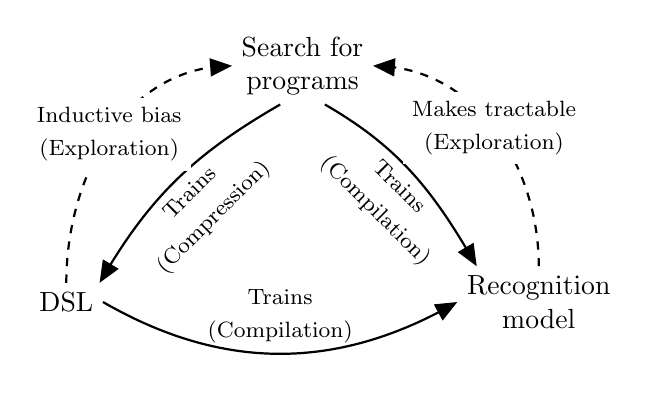
\begin{tikzpicture}
    \begin{scope}[shift = {(1,-1)}]
    \node[align = center](synthesis) at (6,4) {Search for \\programs};
    \node[align = center](DSL) at (3,1) {DSL};
    \node[align = center](recognitionModel) at (9,1) {Recognition \\model};

    \draw [->,thick] (synthesis.-120) to[out = -150,in = 60] node[below,rotate = 45,align = center]{{\footnotesize Trains}\\{\footnotesize (Compression)}} (DSL.30);
    \draw [->,thick] (synthesis.-60) to[out = -30,in = 120] node[below,rotate=-45,align = center]{{\footnotesize Trains}\\{\footnotesize (Compilation)}} (recognitionModel.150);
    \draw [->,thick] (DSL.east) to[out = -30,in = 210] node[above, align = center]{{\footnotesize Trains}\\{\footnotesize (Compilation)}} (recognitionModel.west);

    \draw [->,thick,dashed] (DSL.north) to[out = 90,in = 180] node[fill=white,align = center]{  \footnotesize{Inductive bias}\\\footnotesize{(Exploration)}} (synthesis.west);
    \draw [->,thick,dashed] (recognitionModel.north) to[out = 90,in = 0] node[fill=white,align = center]{{\footnotesize Makes tractable}\\{\footnotesize (Exploration)}} (synthesis.east);
  \end{scope}
    \end{tikzpicture}
  \caption{\system solves for programs, the DSL, and a neural network (recognition model). Each of these steps iteratively bootstraps off of the others.}  \label{feeding}\vspace{-0.4cm}
\end{wrapfigure}
  \end{comment}
\\\noindent \textbf{Exploration: Searching for programs.}  Our program search
is informed by both the DSL and the recognition model. When these
improve, we can solve more tasks.
\\\noindent\textbf{Compression: Improving the DSL.} We induce the DSL
from the programs found in the exploration phase, aiming
to maximally compress (or, raise the prior probability of) these
programs.  As we solve more tasks, we hone in on DSLs that
more closely match the domain.
\\\noindent \textbf{Compilation: Learning a neural recognition model.}  We
update the recognition model by training on two data sources: samples
from the DSL (as in the Helmholtz Machine's ``sleep'' phase), and
programs found by the search procedure during exploration. As the DSL
improves and as search finds more programs, the recognition model gets
more data to train on, and better data.


\begin{comment}
Sec.~\ref{mathematicalFraming} frames this 3-step procedure as probabilistic inference.
Sec.~\ref{explorationSection} explains how we search for programs that solve the tasks;
Sec.~\ref{recognitionSection} explains how we train a neural network to  search for programs; and
Sec.~\ref{grammarInductionSection} explains how we induce a DSL from programs.
  \end{comment}
\subsection{Hierarchical Bayesian Framing}\label{mathematicalFraming}

\system takes as input a set of \emph{tasks}, written $X$, each of which is a program synthesis problem.
It has at its disposal a domain-specific \emph{likelihood model}, written $\probability[x|p]$, which scores the likelihood of a task $x\in X$ given a program $p$.\footnote{For example, for string editing,
  the likelihood is 1 if the program predicts the observed outputs on the observed inputs,
and 0 otherwise.}
Its goal is to solve each of the tasks by writing a program,
and also to infer a DSL, written $\mathcal{D}$.
We equip $\mathcal{D}$ with a real-valued weight vector $\theta$, and together
$(\mathcal{D},\theta)$ define a generative model over programs.
We frame our goal as maximum a posteriori (MAP) inference of $(\mathcal{D},\theta)$ given $X$.
Writing $J$ for the joint probability of $(\mathcal{D},\theta)$ and $X$, we want the $\mathcal{D}^*$ and $\theta^*$ solving:
\begin{align}\label{intractableObjectives}
\nonumber  J(\mathcal{D},\theta)\triangleq \probability[\mathcal{D},\theta]\prod_{x\in X} \sum_p \probability[x|p]\probability[p|\mathcal{D},\theta]\\
  \mathcal{D}^* = \argmax_{\mathcal{D}}\int J(\mathcal{D},\theta)\;\mathrm{d}\theta \qquad
  \theta^* =\argmax_\theta J(\mathcal{D}^*,\theta)
\end{align}

%% Inference in this model is
%% difficult because the programs are unobserved,
%% and so we must solve a hard search problem to recover them. To make
%% search tractable we learn a bottom-up \emph{recognition
%%   model} (written $q(\cdot )$, Fig.~\ref{graphicalModel}(b)).
%% The recognition model $q(\cdot )$ is a neural
%% network that regresses from input/output pairs to a distribution over
%% programs likely to explain the input/outputs. We can also view $q(\cdot )$ as implementing an amortized
%% inference
%% scheme~\cite{le2016inference}.
%%  The neural recognition model and the
%% generative model embodied in the DSL jointly train each other, as they
%% iteratively learn to solve more programming tasks.



The above equations summarize the problem from the point of view of an ideal Bayesian learner.
However, Eq.~\ref{intractableObjectives}
is wildly intractable because evaluating $J(\mathcal{D},\theta)$ involves
summing over the  infinite set of all programs.
In practice we will only ever be able to sum over a finite set of programs.
So, for each task, we define a finite set of programs, called a \emph{frontier}, and only marginalize over the frontiers:
\\\noindent\textbf{Definition.} A \emph{frontier of task $x$}, written $\mathcal{F}_x$,
is a finite set of programs s.t. $\probability[x|p] > 0$ for all $p\in \mathcal{F}_x$.

Using the frontiers we  define the following intuitive lower bound on the joint probability, called $\lowerBound$:
\begin{align}
 J\geq \lowerBound\triangleq\probability[\mathcal{D},\theta]\prod_{x\in X} \sum_{p\in \mathcal{F}_x} \probability[x|p]\probability[p|\mathcal{D},\theta]
\end{align}

%% If we had a $(\mathcal{D},\theta)$ solving Eq.~\ref{intractableObjectives}, then we could recover the most likely program for task $x$ by maximizing $\probability[x|p] \probability[p|\mathcal{D},\theta]$.
%% Through this lens we now take as our goal to solve Eq.~\ref{intractableObjectives}.
%% But even \emph{evaluating} Eq.~\ref{intractableObjectives} is intractable because it involves summing over the infinite set of all possible programs, as an ideal Bayesian learner would.
%% In practice, we must instead marginalize over
%% some finite set of programs.

%% In general, programs are hard-won: finding even a single program that explains a given observation presents a daunting combinatorial search problem.

%% Now in theory we would like to sum over the entire infinite space
%% of all programs -- but this is of course impossible.

%% In general this marginalization over $\theta$ is intractable, so we make an AIC-style approximation\footnote{Sec.~\ref{grammarInductionSection} explains that $\mathcal{D}$ is a context-sensitive grammar.
%% Conventional natural-language processing (NLP) approaches to using variational inference to lower bound the marginal over $\theta$ do not apply in our setting.}, $A\approx \log\probability[\mathcal{D}|X] $:
%% \begin{align}
%%   A =   \log \probability[\mathcal{D}] + \argmax_{\theta}& \sum_{x\in X}\log \sum_p\probability[x|p]\probability[p|\mathcal{D},\theta]\nonumber\\
%% &+  \log P(\theta|\mathcal{D}) - ||\theta||_0 \label{AIC}
%%   \end{align}
\system does approximate MAP inference  by maximizing this lower bound on the joint probability,
alternating maximization w.r.t. the frontiers (Exploration) and the DSL (Compression):
\\\noindent \textbf{Program Search: Maxing $\lowerBound$ w.r.t. the frontiers.} Here $(\mathcal{D},\theta)$ is fixed and we
want to find new programs to add to  the frontiers so that $\lowerBound$ increases the most.
$\lowerBound$ most increases by finding programs where $\probability[x,p|\mathcal{D},\theta]$
is large.
%% which we can accomplish by adding new programs to the frontiers means searching for new programs $p$ for task $x$
%% where  is large.
\\\noindent \textbf{DSL Induction: Maxing $\int \lowerBound\;\mathrm{d}\theta$ w.r.t. the DSL.} Here $\left\{\mathcal{F}_x \right\}_{x\in X}$ is held fixed, and so we can evaluate $\lowerBound$. Now the problem is that of searching the discrete space of DSLs and finding one maximizing $\int \lowerBound\;\mathrm{d}\theta$.
Once we have a DSL $\mathcal{D}$ we can update $\theta$ to $\argmax_\theta \lowerBound(\mathcal{D},\theta,\left\{\mathcal{F}_x \right\})$. 


Searching for programs is hard because
of the large combinatorial search space. We ease this difficulty by training a neural recognition model, $q(\cdot |\cdot )$,
during the compilation phase: $q$ is trained to approximate the
posterior over programs, $q(p|x)\approx \probability[p|x,\mathcal{D},\theta}]\propto\probability[x|p]\probability[p|\mathcal{D},\theta}]$,
  thus amortizing the cost of finding programs with high posterior probability.

\textbf{Neural recognition model: tractably maxing $\lowerBound$ w.r.t. the
  frontiers.}  Here we train %% a neural network, $q$, to predict a
%% distribution over programs conditioned on a task. The objective of $q$
%% is
$q(p|x)$ to assign high probability to programs $p$ where
$\probability[x,p|\mathcal{D},\theta]$ is large, because including those programs
in the frontiers will most increase $\lowerBound$.  %% With $q$ in hand we can find programs for
%% the frontier $\mathcal{F}_x$ by searching for programs that maximize
%% $q(p|x)$.
%% Rather than directly predicting a distribution over $p$ conditioned on $x$,
%% the recognition model predicts a distribution $\theta^{(x)}$ over components of the DSL.
%% This taps into the intuition that programming is primarily a top-down activity:
%% as human programmers, we often first decide what kind of
%% programming constructs we might need to use,
%% and then we figure out how to assemble them in to the desired program.
%% This approach implements an amortized
%% inference scheme~\cite{le2016inference,ritchie2016deep} for the generative model in
%% Fig.~\ref{graphicalModel}.




%% Learning the DSL eases the difficulty of synthesis
%% by exposing a domain-specific basis for constructing programs.
%% Another complementary means of meeting search is to learn a
%% bottom-up \emph{recognition model}

\subsection{Exploration: Searching for Programs}\label{explorationSection}

Now our goal is to search for programs solving the tasks.  We use the simple approach of enumerating programs from
the DSL  in decreasing order of their probability,
and then checking if a program $p$ assigns positive
probability to a task ($\probability[x|p] > 0$); if so, we incorporate $p$ 
into the frontier $\mathcal{F}_x$.

To make this concrete we need to define what programs actually are and
what form $\probability[p |\mathcal{D},\theta]$ takes.
We represent programs as $\lambda$-calculus expressions.
$\lambda$-calculus is a formalism for expressing functional programs
that closely resembles Lisp,
including variables, function application, and the ability to create new functions.
Throughout this paper we will write $\lambda$-calculus expressions in Lisp syntax.
Our programs are all strongly typed.
We use the Hindley-Milner polymorphic typing system~\cite{pierce} which is
used in functional programming languages like OCaml and Haskell.
%% Type variables are always written using lowercase Greek letters
%% and we write $\alpha\to \beta$ to mean a function that takes an input of type $\alpha$
%% and returns something of type $\beta$.
%% We use the notation $p:\tau$ to mean that the $\lambda$-calculus expression $p$
%% has the type $\tau$.
%% For example, to describe the type of the identity function
%% we would say \code{(lambda (x) x)}$:\alpha\to \alpha$.
%% We say a type $\alpha$ \emph{unifies} with $\tau$ if every expression
%% $p:\alpha$ also satisfies $p:\tau$. Furthermore, the act of \emph{unifying}
%% a type $\alpha$ with $\tau$ is to introduce constraints on the type
%% variables of $\alpha$ to ensure that $\alpha$ unifies with $\tau$.
%% See Supplement for more detail on program representation.
We now define DSLs:

\noindent\textbf{Definition: $(\mathcal{D},\theta)$.}
A DSL $\mathcal{D}$ is a set of typed $\lambda$-calculus expressions.
%\\\noindent\textbf{Definition.}
A weight vector $\theta$ for a DSL $\mathcal{D}$ is a vector of $|\mathcal{D}| + 1$ real numbers:
one number for each DSL element $e\in \mathcal{D}$, written $\theta_e$ and controlling the probability of  $e$ occurring in a program,
and a weight controlling the probability of a variable occurring in a program, $\theta_{\text{var}}$.

Together with its weight vector,
a DSL defines a distribution over programs, $\probability[p|\mathcal{D},\theta]$.
In the supplement, we define this distribution  
by specifying a procedure for drawing samples from $\probability[p|\mathcal{D},\theta]$. Care must be taken to ensure that programs are well-typed
and that variable scoping rules are obeyed.
With this distribution in hand, we search for programs by enumerating
$\lambda$-calculus expressions in decreasing order of their probability under
$(\mathcal{D},\theta)$.


Why enumerate, when the program synthesis community has invented many
sophisticated algorithms that search for programs?~\cite{solar2008program,schkufza2013stochastic,feser2015synthesizing,osera2015type,polozov2015flashmeta}.
We have two reasons:
(1) A key point of our work is that learning the DSL, along with a neural recognition model, can make program induction tractable, even if the search algorithm is very simple.
(2) Enumeration is a general approach that can be applied to any program induction problem. Many of these more sophisticated approaches require special conditions on
  the space of  programs.

  A drawback of using an enumerative search algorithm is that we have no
efficient means of solving for arbitrary constants that might occur in the
program. In Sec.~\ref{regressionSection},
we will show how to find programs with real-valued constants
by automatically differentiating through the program and setting the constants using gradient descent.
%% In Sec.~\ref{textSection}
%% we will show that the bottom-up neural recognition model can learn
%% which discrete constants should be included in a program.







\subsection{Compilation: Learning a Neural Recognition Model}\label{recognitionSection}

The purpose of training the recognition model is to amortize the cost of searching for
programs.  It does this by learning to predict, for each task,
programs with high likelihood according to 
$\probability[x|p]$ while also being
probable under the prior $(\mathcal{D},\theta)$.  Concretely,
the recognition model $q$ predicts, for each
task $x\in X$, a weight vector $q(x) = \theta^{(x)}\in
\mathbb{R}^{|\mathcal{D}| + 1}$.  Together with the DSL, this defines
a distribution over programs, $\probability[p|\mathcal{D},\theta =
  q(x)]$.  We abbreviate this distribution as $q(p|x)$.  The crucial
aspect of this framing is that the neural network leverages the
structure of the learned DSL, so it is \emph{not} responsible for
generating programs wholesale.  We share this aspect with
DeepCoder~\cite{balog2016deepcoder} and~\cite{menon2013machine}.

How should we get the data to train $q$?
This is nonobvious  because \system is only weakly supervised (i.e., learns only from tasks and not from (program, task) pairs).
One approach is to sample programs from the DSL,
run them to get their input/outputs,
and then train $q$ to predict the program from the input/outputs.
This approach is like how a Helmholtz machine
trains its recognition model during its ``sleep'' phase~\cite{dayan1995helmholtz}.
The advantage of ``Helmholtz machine'' training is that
we can draw unlimited samples from the DSL,
training on a large amount of data.
Another approach is
 self-supervised learning,
training $q$ on the (program, task)
pairs discovered by the algorithm so far.
The advantage of self-supervised learning
is that the training data is much higher quality,
because we are training on the actual tasks.
Due to these complementary advantages,
we train on both these sources of data.

Formally, $q$ should approximate the true posteriors over programs: minimizing the expected KL-divergence, $  \expect\left[\text{KL}\left(\probability[p|x,\mathcal{D},\theta]\|q(p|x) \right) \right]$,
 equivalently maximizing $  \expect[\sum_p\probability[p|x,\mathcal{D},\theta]\log q(p|x) ]$,
%% \begin{equation*}
%%   \expect\left[\sum_p\probability[p|x,\mathcal{D},\theta]\log q(p|x) \right]
%% \end{equation*}
 where the expectation is taken over tasks. Taking this expectation over the empirical distribution of tasks gives self-supervised training; taking it over samples from the generative model gives  Helmholtz-machine style training.
 The  objective for a recognition model ($\mathcal{L}_{\text{RM}}$) combines the Helmholtz machine ($\mathcal{L}_{\text{HM}}$) and self supervised ($\mathcal{L}_{\text{SS}}$) objectives, $\mathcal{L}_{\text{RM}} = \mathcal{L}_\text{SS} + \mathcal{L}_\text{HM}$:
\begin{align}\nonumber
\mathcal{L}_{\text{HM}} = \expect_{(p,x)\sim(\mathcal{D},\theta) }\left[\log q(p|x)\right]\quad
\mathcal{L}_{\text{SS}} = \expect_{x\sim X}\left[\sum_{p\in \mathcal{F}_x}
  \frac{\probability\left[x,p|\mathcal{D},\theta \right]}{\sum_{p'\in \mathcal{F}_x}\probability\left[x,p'|\mathcal{D},\theta \right]}\log q(p|x)\right]
\end{align}
\begin{comment}
  The $\mathcal{L}_{\text{HM}}$ objective is essential for data efficiency:
all of our experiments train \system on only a few hundred tasks, which is too little for
a high-capacity neural network $q$.
Once we bootstrap a $(\mathcal{D},\theta)$,
we can draw unlimited samples from $(\mathcal{D},\theta)$
and train $q$ on those samples.
  \end{comment}
Evaluating $\mathcal{L}_{\text{HM}}$ involves sampling programs from
the current DSL, running them to get their outputs,
and then training $q$ to regress from the input/outputs to the program.
Since these programs map inputs to outputs,
we need to sample the inputs as well.
Our solution is to sample the inputs
from the empirical observed distribution of inputs in $X$.

%% The architecture of $q$ depends upon the domain.  For domains with
%% sequential structure like strings and lists, we use an RNN to encode
%% each input/output example.  For domains with fixed-dimensionality
%% inputs/outputs we use a multilayer perceptron.  We MaxPool across all
%% of the input/output examples. See Supplement for details.

\subsection{Compression: Learning a Generative Model (a DSL)}\label{grammarInductionSection}

The purpose of the DSL is to
offer a set of abstractions
that allow an agent to easily express solutions to the tasks at hand.
%In the \system algorithm we infer the DSL from a collection of frontiers.
Intuitively, we want the algorithm to
look at  the frontiers and
generalize beyond them, 
both so the DSL can better express the current solutions,
and  also so that the DSL might expose new abstractions
which will later be used to
discover more programs.
 Formally, we want the DSL maximizing $\int \lowerBound\;\mathrm{d}\theta$ (Sec.~\ref{mathematicalFraming}).
We replace this marginal with an AIC approximation, giving the following objective for DSL induction:
\begin{equation}
      \log \probability[\mathcal{D}] + \argmax_{\theta}\sum_{x\in X}\log \sum_{p\in \mathcal{F}_x}\probability[x|p]\probability[p|\mathcal{D},\theta] + \log \probability[\theta|\mathcal{D}] - \|\theta\|_0 \label{AIC}
  \end{equation}
We induce a DSL by searching locally through the space of DSLs,
proposing small changes to $\mathcal{D}$ until Eq.~\ref{AIC} fails to increase.
The search moves work by introducing new
$\lambda$-expressions into the DSL.
We propose these new expressions by extracting subexpressions from
programs already in the frontiers.
These subexpressions
are fragments of the original programs, and can introduce new variables (Fig.~\ref{fragmentExample}),
which then become new functions in the DSL.
The idea of storing and reusing
fragments of expressions comes from Fragment Grammars~\cite{tim} and Tree-Substitution Grammars~\cite{cohn2010inducing}.



To define the prior distribution over $(\mathcal{D},\theta})$, we penalize the syntactic complexity of the $\lambda$-calculus expressions in the DSL, defining $    \probability[\mathcal{D}]\propto\exp\left(-\lambda\sum_{p\in \mathcal{D}}\text{size}(p) \right)$ where $\text{size}(p)$  measures the size of the syntax tree of program $p$,
and place a symmetric Dirichlet prior over the weight vector $\theta$.
%% , $  \probability[\theta|\mathcal{D}] = \text{Dir}(\theta|\alpha)$, where
 %% $\alpha$ is a concentration parameter controlling the smoothness of the prior over $\theta$.
%Alg.~\ref{grammarInductionAlgorithm} specifies the DSL induction algorithm.

\begin{wrapfigure}{R}{0.6\textwidth}\vspace{-0.7cm}
  \begin{minipage}{0.6\textwidth}    
    \begin{algorithm}[H]
      \caption{The \system Algorithm}
      \label{mainAlgorithm}
      \begin{algorithmic}
        \STATE {\bfseries Input:} Initial DSL $\mathcal{D}$, set of tasks $X$, iterations $I$
        \STATE \textbf{Hyperparameters:} Enumeration timeout $T$
        %     \STATE \textbf{Output:} DSL $\mathcal{D}$, weight vector $\theta$, recognition model $q(\cdot)$
        \STATE Initialize $\theta\gets \text{uniform}$ %, $q_0(\cdot ) = \theta_0$
        \FOR{$i=1$ {\bfseries to} $I$}
        %     \FOR{$x:\tau\in X$}
        \STATE  $\mathcal{F}^{\theta}_x\gets \{p| p\in \text{enum}(\mathcal{D},\theta,T)\text{ if }\probability[x|p] > 0\}$ \footnotesize{(\textbf{Explore})}
        \STATE $q\gets \text{train recognition model, maximizing }\mathcal{L}_{\text{RM}}$ \hspace{0.2cm}(\footnotesize{\textbf{Compile}})
        \STATE  $\mathcal{F}^{q}_x\gets\{p|p\in \text{enum}(\mathcal{D},q(x),T)\text{ if }\probability[x|p] > 0\}$ \footnotesize{\textbf{(Explore)}}
        
        \STATE $\mathcal{D},\theta\gets $induceDSL$(\{\mathcal{F}^{\theta}_x\cup\mathcal{F}^{q}_x\}_{x\in X})$  \hspace{1.1cm} \footnotesize{\textbf{(Compress)}}
        %% \STATE Define $Q_x(z) \propto \begin{cases}
        %%   \probability[x|z]\probability[z|\mathcal{D}_i,\theta_i]&x\in \mathcal{F}_x\\
        %%   0&x\not \in \mathcal{F}_x
        %% \end{cases}
        \ENDFOR
        \STATE \textbf{return} $\mathcal{D},\theta,q$
      \end{algorithmic}
    \end{algorithm}
  \end{minipage}
\vspace{-0.7cm}\end{wrapfigure}%% To appropriately score each proposed $\mathcal{D}$ we must reestimate the weight vector $\theta$.
%% Although this  may seem 
%% very similar to estimating the parameters of a probabilistic context free grammar,
%% for which we have effective approaches like the Inside/Outside algorithm~\cite{international2000derivation},
%% our DSLs are context-sensitive due to the presence of variables
%% in the programs and also due to the polymorphic typing system.
%% In the Supplement we derive a tractable MAP estimator for $\theta$.
Putting all these ingredients together, Alg.~\ref{mainAlgorithm} describes how we combine program search,
recognition model training, and DSL induction.
\begin{figure*}
\centering  \begin{tabular}{ll}
    \toprule
    Example programs in frontiers&Proposed subexpression\\\midrule
    \begin{tabular}{l}
      \code{(lambda (a b) (foldr b (cons "," a)}\\
      \phantom{\code{(lambda }}\code{(lambda (x z) (cons x z))))}\\
      \code{(lambda (a b) (foldr a b (lambda (x z) (cons x z))))}
    \end{tabular}&
    \begin{tabular}{l}
      \code{(foldr a b (lambda (x z) }\\
      \phantom{\code{(foldr a b }}\code{(cons x z)))}
      \end{tabular}
\\\bottomrule
  \end{tabular}
  \caption{The DSL induction algorithm proposes subexpressions of programs to add to the DSL.
    These subexpressions are taken from programs in the frontiers (left column), and can introduce new variables (right column: \code{a} and \code{b}). Here, the proposed subexpression appends two lists.} 
  \label{fragmentExample}
\end{figure*}

\begin{comment}
\subsection{Implementing \system}

Alg.~\ref{mainAlgorithm} describes how we combine program search,
recognition model training, and DSL induction.
We note the following implementation details:
(1) We perform an exploration cycle before each compression and compilation  cycle.
(2) On the first iteration, we do \emph{not} train the recognition model on samples from
the generative model because a generative model has not yet been learned --
we instead train the network to only maximize $\mathcal{L}_{\text{AE}}$.
%% (3) Because the frontiers can grow very large,
%% we only keep around the top $10^4$ programs $p$ in each frontier $\mathcal{F}_x$
%% with the highest likelihood $\probability[x,p|\mathcal{D},\theta]$.
(3) During both DSL induction and neural net training, we calculate Eq.~\ref{AIC} and $\mathcal{L}_{\text{RM}}$
by only summing over the top $K$
programs in $\mathcal{F}_x$ as measured by $\probability[x,p|\mathcal{D},\theta]$ -- we found that $K = 2$ sufficed.
(4) For added robustness, we enumerate programs from both the generative model $(\mathcal{D},\theta)$ and the recognition model.
\end{comment}



%\section{Experiments}
%% We first present our experimental results qualitatively,
%% illustrating the learned DSLs.
%% We then show quantitative results (Sec.~\ref{quantitative})
%% comparing \system with lesioned versions
%% of our model that are analogous to prior work.


\section{Sequence manipulating programs}\label{sequences}
We apply \system to list processing (Section~\ref{listSection}) and text editing (Section~\ref{textSection}).
For both these domains we use a bidirectional GRU~\cite{cho2014learning} for the recognition model,
and initially provide the system with a generic
set of list processing primitives: \code{foldr}, \code{unfold}, \code{if}, \code{map}, \code{length}, \code{index}, \code{=}, \code{+}, \code{-}, \code{0}, \code{1}, \code{cons}, \code{car}, \code{cdr}, \code{nil}, and \code{is-nil}.



\subsection{List Functions}\label{listSection}
Synthesizing programs that manipulate data structures is
a widely studied problem in the programming languages community~\cite{feser2015synthesizing}.
%with applications to computer aided programming~\cite{solar2008program}.
We consider this problem within the context of
learning functions that manipulate lists.
We created 244 Lisp-style list manipulation tasks,
each with 15 input/output examples (Tbl.~\ref{listexamples}).
Our data set is challenging along two dimensions:
many of the functions are very complicated,
and the agent must learn to solve these complicated problems from only 244 tasks.
Our data set primarily consists of arithmetic operations upon sequences,
and so, in addition to the Lisp primitives provided for the text editing experiments, we additionally start the system out with the following primitives:
\code{mod}, \code{*}, \code{>}, \code{is-square}, \code{is-prime}, \code{2},
\code{3}, \code{4}, \code{5}.

A complete repertoire of higher-order functions is a staple of functional programming standard libraries.
Although we provided \system with some of the standard higher-order functions,
like \code{foldr} and \code{unfold},
we did not include others.
When trained on these list functions,
our system rediscovers
and then reuses the higher-order function \code{filter} \textbf{Lucas: not sure if it actually does this! It would be cool if we can write something like this though.}


%% Our list function domain consists of hand-designed concepts from which we
%% sample tasks, so there is no ``ground truth'' formal DSL from which these
%% tasks are generated. Additionally, few of these tasks are concatenative ---
%% many of them represent distinct operations.
%% Tasks in this domain are solved by functions that take as input an integer
%% or a list of integers, and have as output either a Boolean, an integer, a
%% list of Booleans, or a list of integers.  There are 225 tasks in total, some
%% of which are shown in Tbl.~\ref{listexamples}.

%% We evaluate \system starting from two different initial DSLs, \emph{base} and
%% \emph{rich}. The base DSL starts with only
%% low-level primitives such as \code{mapi}, \code{reducei}, and
%% \code{if}, whereas the rich DSL includes some common structure that can be
%% built from these such as \code{all}, \code{filter}, \code{slice}, and
%% \code{index}.
%% Both are capable of solving all tasks supplied by our dataset.
%% See Supplement for details on these DSLs.

%% We found  this domain  difficult to tackle without starting from 
%% the rich DSL. Our
%% algorithm, like human learners, requires a spectrum of problems ranging from
%% easy to hard.
%% When starting with the base DSL,
%% we found that there were not enough steppingstones in the curriculum to
%% get \system off the ground.

%The behavior with the base DSL illustrates this phenomena  because the initial set of
%primitives is not paired with a sufficiently large and graded curriculum.


\begin{comment}
\begin{table}
\centering
\begin{tabular}{lll}
  \toprule
  Name & Input & Output \\\midrule
  append-4 & [7\, 0\, 2] & [7\, 0\, 2\, 4] \\
  len & [3\, 5\, 12\, 1] & 4 \\
  has-2 & [4\, 5\, 7\, 4] & \code{false} \\
  repeat-2 & [7\, 0] & [7\, 0\, 7\, 0] \\
  drop-3 & [0\, 3\, 8\, 6\, 4] & [6\, 4] \\
  count-head-in-tail & [1\, 2\, 1\, 1\, 3] & 2 \\
  rotate-2 & [8\, 14\, 1\, 9] & [1\, 9\, 8\, 14] \\
  pow-3 & [10\, 4\, 13] & [1000\, 64\, 2197] \\
  keep-mod-5 & [5\, 9\, 14\, 6\, 3\, 0] & [5\, 0] \\
  \bottomrule
\end{tabular}
\caption{Sample tasks from our list function domain %% We used 15 input/output
  %% examples for each task to reduce ambiguity in the task's function,
  %% ensuring solutions achieve the desired concept.
}
\label{listexamples}
\end{table}

\begin{table}[t]
  \centering
  \begin{tabular}{l}
    \toprule
    $f_0($\code{i$,\ell$}$) \,=\, $\code{(singleton (index i $\ell$))}\\
    \hspace{0.5cm}($f_0$: \emph{Put the $i$-th index into a list})\\
    $f_1($\code{i$,\ell$}$) \,=\, $\code{(++ $\ell$ ($f_0$ i $\ell$))}\\
    \hspace{0.5cm}($f_1$: \emph{Append the $i$-th index})\\
    $f_2($\code{n$,\ell$}$) \,=\, $\code{(any (lambda (x) (= n x)) $\ell$)}\\
    \hspace{0.5cm}($f_1$: \emph{Whether $n$ appears in the list})\\
    $f_3($\code{i$,\ell$}$) \,=\, $\code{(index (negate i) (sort $\ell$))}\\
    \hspace{0.5cm}($f_3$: \emph{Get the $i$-th largest number})\\
    $f_4($\code{n$,\ell$}$) \,=\, $\code{(mapi (lambda (i x) (mod x n)) $\ell$)}\\
    $f_5($\code{k$,\ell$}$) \,=\, $\code{(mapi (lambda (i x) (+ x k)) $\ell$)}\\
    $f_6($\code{k$,$n$,\ell$}$) \,=\, $\code{($f_4$ n ($f_5$ k $\ell$)}\\
    \hspace{0.5cm}($f_6$: \emph{Caesar shift of $k$ in integers modulo $n$})\\
  \bottomrule
  \end{tabular}
  \caption{Some learned DSL primitives for list functions}\label{listinduced}
\end{table}

  \end{comment}

\subsection{String Editing}\label{textSection}
Synthesizing programs that manipulate strings is a classic problem in the
programming languages and AI literatures~\cite{menon2013machine,lau2001programming},
and algorithms that learn string editing programs ship in Microsoft Excel~\cite{gulwani2011automating}.
This prior work presumes a ready-made DSL,
expertly crafted to suit string editing.
We show \system can instead start out with generic Lisp primitives
and recover many of the higher-level building blocks that have made these
other system successful.
An obstacle here, however,
is that
our enumerative search procedure
has no means of generating string constants,
and so we incorporate  string-valued parameters as a primitive,
  defining $\probability[x|p]$ by marginalizing out the
  values of the string via dynamic programming.
  In  Section~\ref{regressionSection},
  we will use a similar trick to synthesize programs containing real numbers using gradient descent.

We automatically generated 109 string editing tasks  %% with 4 input/output examples each
(Fig.~\ref{exampleTextProblem}) and model strings as lists of characters.
At first, \system cannot find any correct programs for most of the tasks.
It assembles a DSL (Tbl.~\ref{textPrimitives}) that lets it rapidly explore the space of programs and find solutions to
all of the tasks.



How well does the  learned DSL generalized to real text-editing scenarios?
We tested, but did not train, our system on problems from the SyGuS~\cite{alur2016sygus} program synthesis competition. Before any learning,
\system solves 32/108 of the problems with an average search time of 11 minutes.
After learning,
it solves 80/108, and does so much faster,
solving them in an average of 29 seconds.
As of the 2017 SyGuS competition,
the best-performing algorithm solves 86/108 problems,
and does so with a
\emph{different hand-engineered DSL for each problem}.
Here  we learned a single DSL
that applied generically to
all of the tasks,
and perform comparably to the best
prior work.


\begin{table}[t]
  \centering
    \begin{tabular}{l}
      \toprule
      $f_0($\code{a}$,$\code{b}$) \,=\, $\code{(foldr a b (lambda (x y) (cons x y))))))}\\
      \hspace{0.5cm}($f_0$: \emph{Appends lists (of characters))}\\
      $f_1($\code{s}$,$\code{c}$) \,=\, $\code{(foldr s s (lambda (x a) (cdr (if (= c x) s a))))}\\
        \hspace{0.5cm}($f_1$: \emph{Drop first characters from }\code{s}\emph{ until  }\code{c}\emph{ reached})\\
      $f_2($\code{s}$) \,=\, $\code{(unfold s empty? car (lambda (z) (}$f_1$\code{ z SPACE)))}\\
        \hspace{0.5cm}($f_2$: \emph{Abbreviates a sequence of words})\\
        $f_3($\code{s}$,$\code{c}$) \,=\, $\code{(foldr s s (lambda (x a) (if (= c x) nil (cons x a))))}\\
        \hspace{0.5cm}($f_3$: \emph{Take characters from }\code{s}\emph{ until }\code{c}\emph{ reached)}
        %(lambda (lambda (fold $0 $0 (lambda (lambda (if (char-eq? $1 $3) empty (cons $1 $0)))))))
  \\\bottomrule
    \end{tabular}
  \caption{Some string editing learned subroutines }\label{textPrimitives}
  \end{table}

\begin{figure}
  \centering\begin{tabular}{r|r}\toprule
Temple Annalisa Haven 185 $\longrightarrow$ TAH1&Nancy FreeHafer $\longrightarrow$ Dr. Nancy\\
Lara Gregori Bradford $\longrightarrow$ LGB& Andrew Cencici $\longrightarrow$ Dr. Andrew
%DkI$>$DwKI$<$xaPoc& 	DWKI\\
%KfvTh$>$Dbl$<$OIJso 	&DBL
\\\midrule
\multicolumn{1}{l|}{$f(\text{\code{s}}) = $\code{(}$f_2$\code{ s)}}&
\multicolumn{1}{l}{$f(\text{\code{s}}) = $\code{(}$f_0$\code{ "Dr. " (}$f_3$\code{ s " "))}}
\\
\bottomrule
  \end{tabular}

  
  %% \vspace{0.25cm}
  
  %% \begin{minipage}{\linewidth}
  %%   \centering
  %%   $f($\code{s}$) \,=\, $
  %% \end{minipage}

  
  \caption{Two string edit tasks (top) and the programs \system writes for them (bottom). $f_0$ and $f_2$ are   subroutines written by \systemEnding, defined in Tbl.~\ref{textPrimitives}.}\label{exampleTextProblem}
\end{figure}


\section{Symbolic Regression: Programs from visual input}\label{regressionSection}
We apply \system
to symbolic regression problems.  Here, the
agent observes points along the curve of a function, and must write a
program that fits those points.  We initially equip our learner with
addition, multiplication, and division, and task it with solving
100 symbolic regression problems, each either a polynomial of degree
1--4 or a rational function.  The recognition model is a
convolutional network that observes an image of the target function's
graph (Fig.~\ref{functions}) -- visually, different kinds of
polynomials and rational functions produce different kinds of graphs,
and so the recognition model can learn to look at a graph and predict
what kind of function best explains it.  A key difficulty, however, is
that these problems are best solved with programs containing real
numbers.  Our solution to this difficulty is to allow the system to
write programs with real-valued parameters, and then fit those
parameters by automatically differentiating through the programs the
system writes and use gradient descent to fit the parameters.
We define the likelihood model, $\probability[x|p]$, by assuming a Gaussian noise model for the input/output examples,
and penalize the use of real-valued parameters using the BIC~\cite{Bishop:2006:PRM:1162264}.

\begin{wrapfigure}{r}{0.3\textwidth} \newcommand{\functionSize}{0.75cm}\vspace{-0.5cm}
  
\includegraphics[width = \functionSize]{figures/functions/0.png}
  
\includegraphics[width = \functionSize]{figures/functions/6.png}
  
\includegraphics[width = \functionSize]{figures/functions/207.png}
  
\includegraphics[width = \functionSize]{figures/functions/160.png}
  
\includegraphics[width = \functionSize]{figures/functions/317.png}\\  
  
\includegraphics[width = \functionSize]{figures/functions/432.png}
  
\includegraphics[width = \functionSize]{figures/functions/415.png}
  
\includegraphics[width = \functionSize]{figures/functions/426.png}
  
\includegraphics[width = \functionSize]{figures/functions/597.png}
  
\includegraphics[width = \functionSize]{figures/functions/591.png}
  \caption{Recognition model input for symbolic regression. While the DSL learns subroutines for rational functions \& polynomials, the recognition  model jointly learns to look at a graph of the function (above) and predict which of those subroutines is appropriate for explaining the observation.}\label{functions}
\end{wrapfigure}
%% \begin{align*}
%%   \log \probability[x|p] \triangleq& \sum_{n\leq N}\log
%%   \mathcal{N}(p(i_n,\vec{\mathcal{R}}^*)|o_n) - \frac{D\log N}{2}
%% \end{align*}

%% %% and integrate over the real-valued parameters, which we collectively write as $\vec{\mathcal{R}}$:
%% %% \begin{align*}
%% %% \log   \probability\left[\{(i_n,o_n)\}|p\right] = \log \int \mathrm{d}\vec{\mathcal{R}}\; P(\vec{\mathcal{R}})\prod_{n\leq N}\mathcal{N}(p(i_n,\vec{\mathcal{R}})|o_n)
%% %% %\text{\emph{BIC:}} &\approx 
%% %% \end{align*}
%% where $\mathcal{N}(\cdot |\cdot )$ is the normal density and
%% $P_{\vec{\mathcal{R}}}(\cdot )$ is a prior over
%% $\vec{\mathcal{R}}$. We approximate this marginal using the BIC~:

%% where $\vec{\mathcal{R}}^*$ is an assignment to $\vec{\mathcal{R}}$
%% found by performing gradient ascent on the likelihood of the
%% observations w.r.t. $\vec{\mathcal{R}}$.

\system learns a DSL containing templates for polynomials of different orders, as well as ratios of polynomials (Fig.~\ref{regressionDSL}).
The algorithm also discovers programs that minimize the number of continuous degrees of freedom.
For example, it learns to represent linear functions with the program
\code{(* real (+ x real))}}, which has two continuous degrees of freedom, and represents quartic functions using the invented DSL primitive $f_6$ in Tbl.~\ref{regressionDSL}
which has five continuous parameters.
This phenomenon arises from our Bayesian framing -- both the bias towards shorter programs and the likelihood model's BIC penalty.
\begin{wrapfigure}{l}{0.35\textwidth}\centering
\begin{tabular}{l}
  \toprule
  $f_0($\code{x}$)\,=\,$\code{(+ x real)}\\
  $f_1($\code{x}$)\,=\,$\code{($f_0$ (* real x))} \\
  $f_2($\code{x}$)\,=\,$\code{($f_1$ (* x (}$f_0$\code{ x)))}\\
  \hspace{0.5cm}\emph{($f_2$: quadratics)}\\
  $f_3($\code{x}$)\,=\,$\code{(/ (}$f_2$\code{ x) (}$f_0$\code{ x))}\\
    \hspace{0.5cm}\emph{($f_3$: ratio of polynomials)}
  \\\bottomrule
\end{tabular}
\caption{Some learned subroutines for symbolic regression. System starts with addition, multiplication, division, and real numbers, and learns to build rational functions and polynomials up to 4th order.}\label{regressionDSL}
\end{wrapfigure}

%% The neural recognition model accelerates inference,
%% but given enough iterations of our algorithm,
%% a lesioned version without the recognition model eventually comes close to catching up (green curves in Fig.~\ref{regressionLearningCurve}; No NN in Tbl.~\ref{regressionComparison}).
%% We compare our model on held-out tasks against 4 baselines (Tbl.~\ref{regressionComparison}).


\subsection{Quantitative Results}\label{quantitative}

We compare  with four baselines on  held-out tasks:
\\\noindent \textbf{Ours (no NN)}, which lesions the recognition model.
\\\noindent \textbf{RF/DC}, which holds the generative model $(\mathcal{D},\theta)$ fixed and learns
a recognition model only from samples from the fixed generative model.
This is equivalent to our algorithm with $\lambda = \infty$ (Sec.~\ref{grammarInductionSection})
and $\mathcal{L}_{\text{RM}} = \mathcal{L}_{\text{HM}}$ (Sec.~\ref{recognitionSection}).
We call this baseline RF/DC because
this setup is closest to how RobustFill~\cite{devlin2017robustfill} and DeepCoder~\cite{balog2016deepcoder} are trained.
We can not compare directly with these systems,
because they are engineered for one specific domain, and 
do not have publicly available code and datasets.
\\\noindent \textbf{PCFG}, which lesions the recognition model, learns $\theta$, and fixes $\mathcal{D}$.
This is equivalent to \system with $q(x) = \theta$ and $\lambda = \infty$,
and is like learning the parameters of a PCFG while not learning its structure.
\\\noindent \textbf{Enum}, which enumerates a frontier without any learning -- equivalently, our first exploration cycle.

For each domain,
we are interested both in how many tasks the
agent can solve and how quickly it can find those solutions.
%% For symbolic regression, we also care about the quality
%% of the solution, as measured by the likelihood model $\probability[x|p]$,
%% e.g. did the agent correctly explain a linear function
%% using two numbers, or did it introduce extraneous parameters?
Tbl.~\ref{baselineComparisons}
compares our model against these baselines.
Our full model consistently
improves on the baselines,
sometimes dramatically (string editing and symbolic regression).
The recognition model 
consistently increases the number of solved held-out tasks,
and lesioning it also slows down the convergence of the algorithm,
taking more iterations to reach a given number of tasks solved (Fig.~\ref{learningCurves}).
This supports a view of the recognition model as a way of amortizing the cost of searching for programs.

\begin{wraptable}{r}{0.6\textwidth}
%% This radically shrinks the table
\tabcolsep=4pt
\renewcommand{\arraystretch}{0.5}
\begin{tabular}{llllll}
  \toprule& Ours& \begin{tabular}{c}
    Ours\\(no NN)
    \end{tabular}& RF/DC & PCFG & Enum

  %% \\\midrule\multicolumn{6}{c}{\emph{Boolean Circuits}}\\\midrule
  %% \% solved &
  %% \textbf{84\%} &76\%& 63\%&62\%&62\%\\
  %% Solve time&  0.9s&  1.1s&1.2s&1.3s&1.3s


  \\\midrule\multicolumn{6}{c}{\emph{List functions}}\\\midrule
  \% solved&\textbf{86\%} &84\% &60\%&74\%&70\%\\
  Solve time&  0.8s&0.7s&1.0s&1.0s&1.1s

  \\\midrule\multicolumn{6}{c}{\emph{String Editing}}\\\midrule
  \% solved&\textbf{75\%} &\% &33\%&0\%&30\%\\
  Solve time&  29s&s&80s&--&

  %% \\\midrule\multicolumn{6}{c}{\emph{List functions (base DSL)}}\\\midrule
  %% \% solved&\textbf{52\%} &\textbf{52\%} &40\%&44\%&42\%\\
  %% Solve time&  0.4s&0.7s&1.2s&0.9s&1.0s

  \\\midrule\multicolumn{6}{c}{\emph{Symbolic Regression}}\\\midrule
  \% solved&   \textbf{84\% }&75\%&38\%&38\%&37\% \\
  Solve time&  24s& 40s  &31s&55s&29s\\
  %% MDL (nats)&   9.3 &11.0&2.3&--&4.6

  \\\bottomrule
  \end{tabular}
\caption{\% solved w/ 5 sec timeout. Solve time: averaged over solved
  tasks.  RF/DC: trained like RobustFill/DeepCoder.  PCFG: model w/o
  structure learning.  Enum: model w/o any learning.  %% MDL:
  %% $-\expect\left[\probability[x|p] \right]$. For domains other than
  %% symbolic regression MDL is 0 nats.
  %% For symbolic regression MDL is a
  %% proxy for \# of continuous parameters.
}\vspace{-0.5cm}\label{baselineComparisons} \end{wraptable}

\begin{figure}\centering
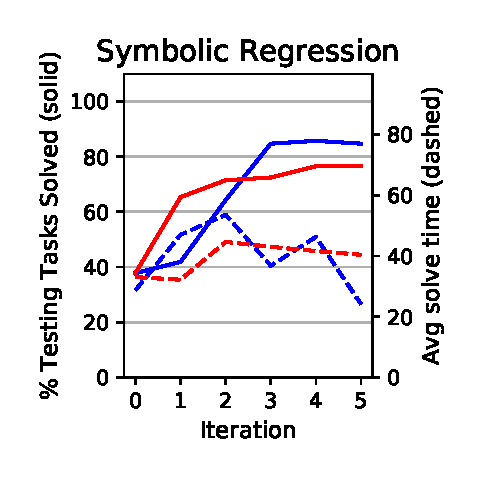
\includegraphics[width = 3.5cm]{figures/rationalCurve.eps} 
  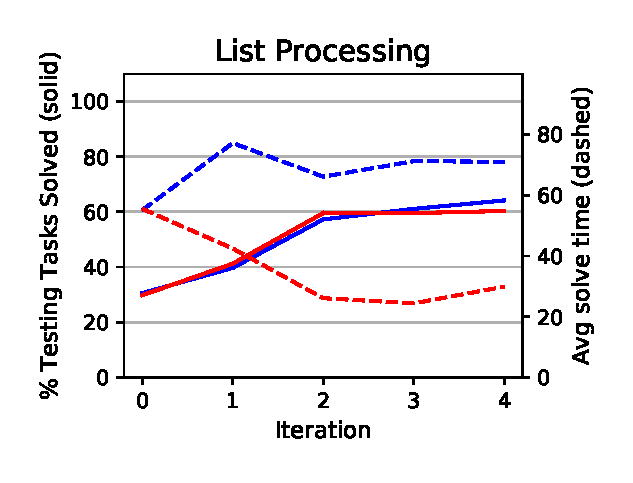
\includegraphics[width = 3.5cm]{figures/list.eps}
  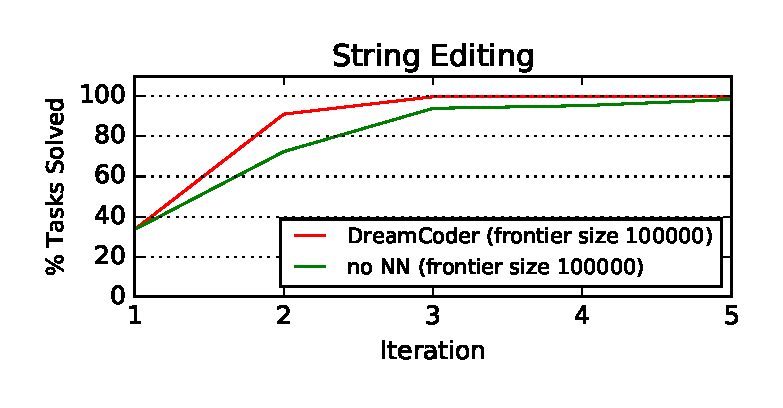
\includegraphics[width = 3.5cm]{figures/textLearningCurve.eps}        
  \caption{Learning curves for \system both with (blue) and without (red) the recognition model as the frontier size is varied (solid/dashed/dotted lines).}\label{learningCurves} 
\end{figure}

\section{Related Work}
 Our work is far from the first for learning to learn programs,
 an idea that goes back to Solomonoff~\cite{solomonoff1989system}:

 \noindent \emph{Deep learning:} Much recent work in the ML community has
 focused on creating neural networks that regress from
 input/output examples to programs~\cite{devlin2017robustfill,devlin2017neural,menon2013machine,balog2016deepcoder}. %This family of work is closest to our RF/DC baseline.
 These neural networks are typically trained with strong supervision (i.e., with annotated ground-truth programs) on massive data sets (i.e., hundreds of millions~\cite{devlin2017robustfill}).
 Our work  considers a weakly-supervised regime where ground truth programs are not provided and
 the agent must learn from a few hundred tasks.
 

 \noindent \emph{Inventing new subroutines for program induction:}
 Several program induction algorithms, most prominently the EC algorithm~\cite{Dechter:2013:BLV:2540128.2540316}, take as their goal to learn new, reusable subroutines that are shared in a multitask setting. We find this work inspiring and motivating,
 and extend it along two dimensions: (1) we propose a new algorithm for
 inducing reusable subroutines, based on Fragment Grammars~\cite{tim};
 and (2) we show how to combine these techniques with bottom-up neural recognition models.
 Other instances of this related idea are~\cite{DBLP:conf/icml/LiangJK10}, Schmidhuber's OOPS model~\cite{schmidhuber2004optimal}, and predicate invention in ILP~\cite{DBLP:conf/ecai/LinDETM14}.
 
 Our work is an instance of
 Bayesian Program
 Learning (BPL; see~\citep{lake2015human,Dechter:2013:BLV:2540128.2540316,ellis2016sampling,DBLP:conf/icml/LiangJK10}). Previous BPL systems have largely assumed a fixed DSL (but see~\cite{DBLP:conf/icml/LiangJK10}),
 and our contribution here is a general way of doing BPL with less hand-engineering of the DSL.
 
 \section{Contribution and Outlook}

\begin{wrapfigure}{r}{0.4\textwidth}
  \begin{center}
    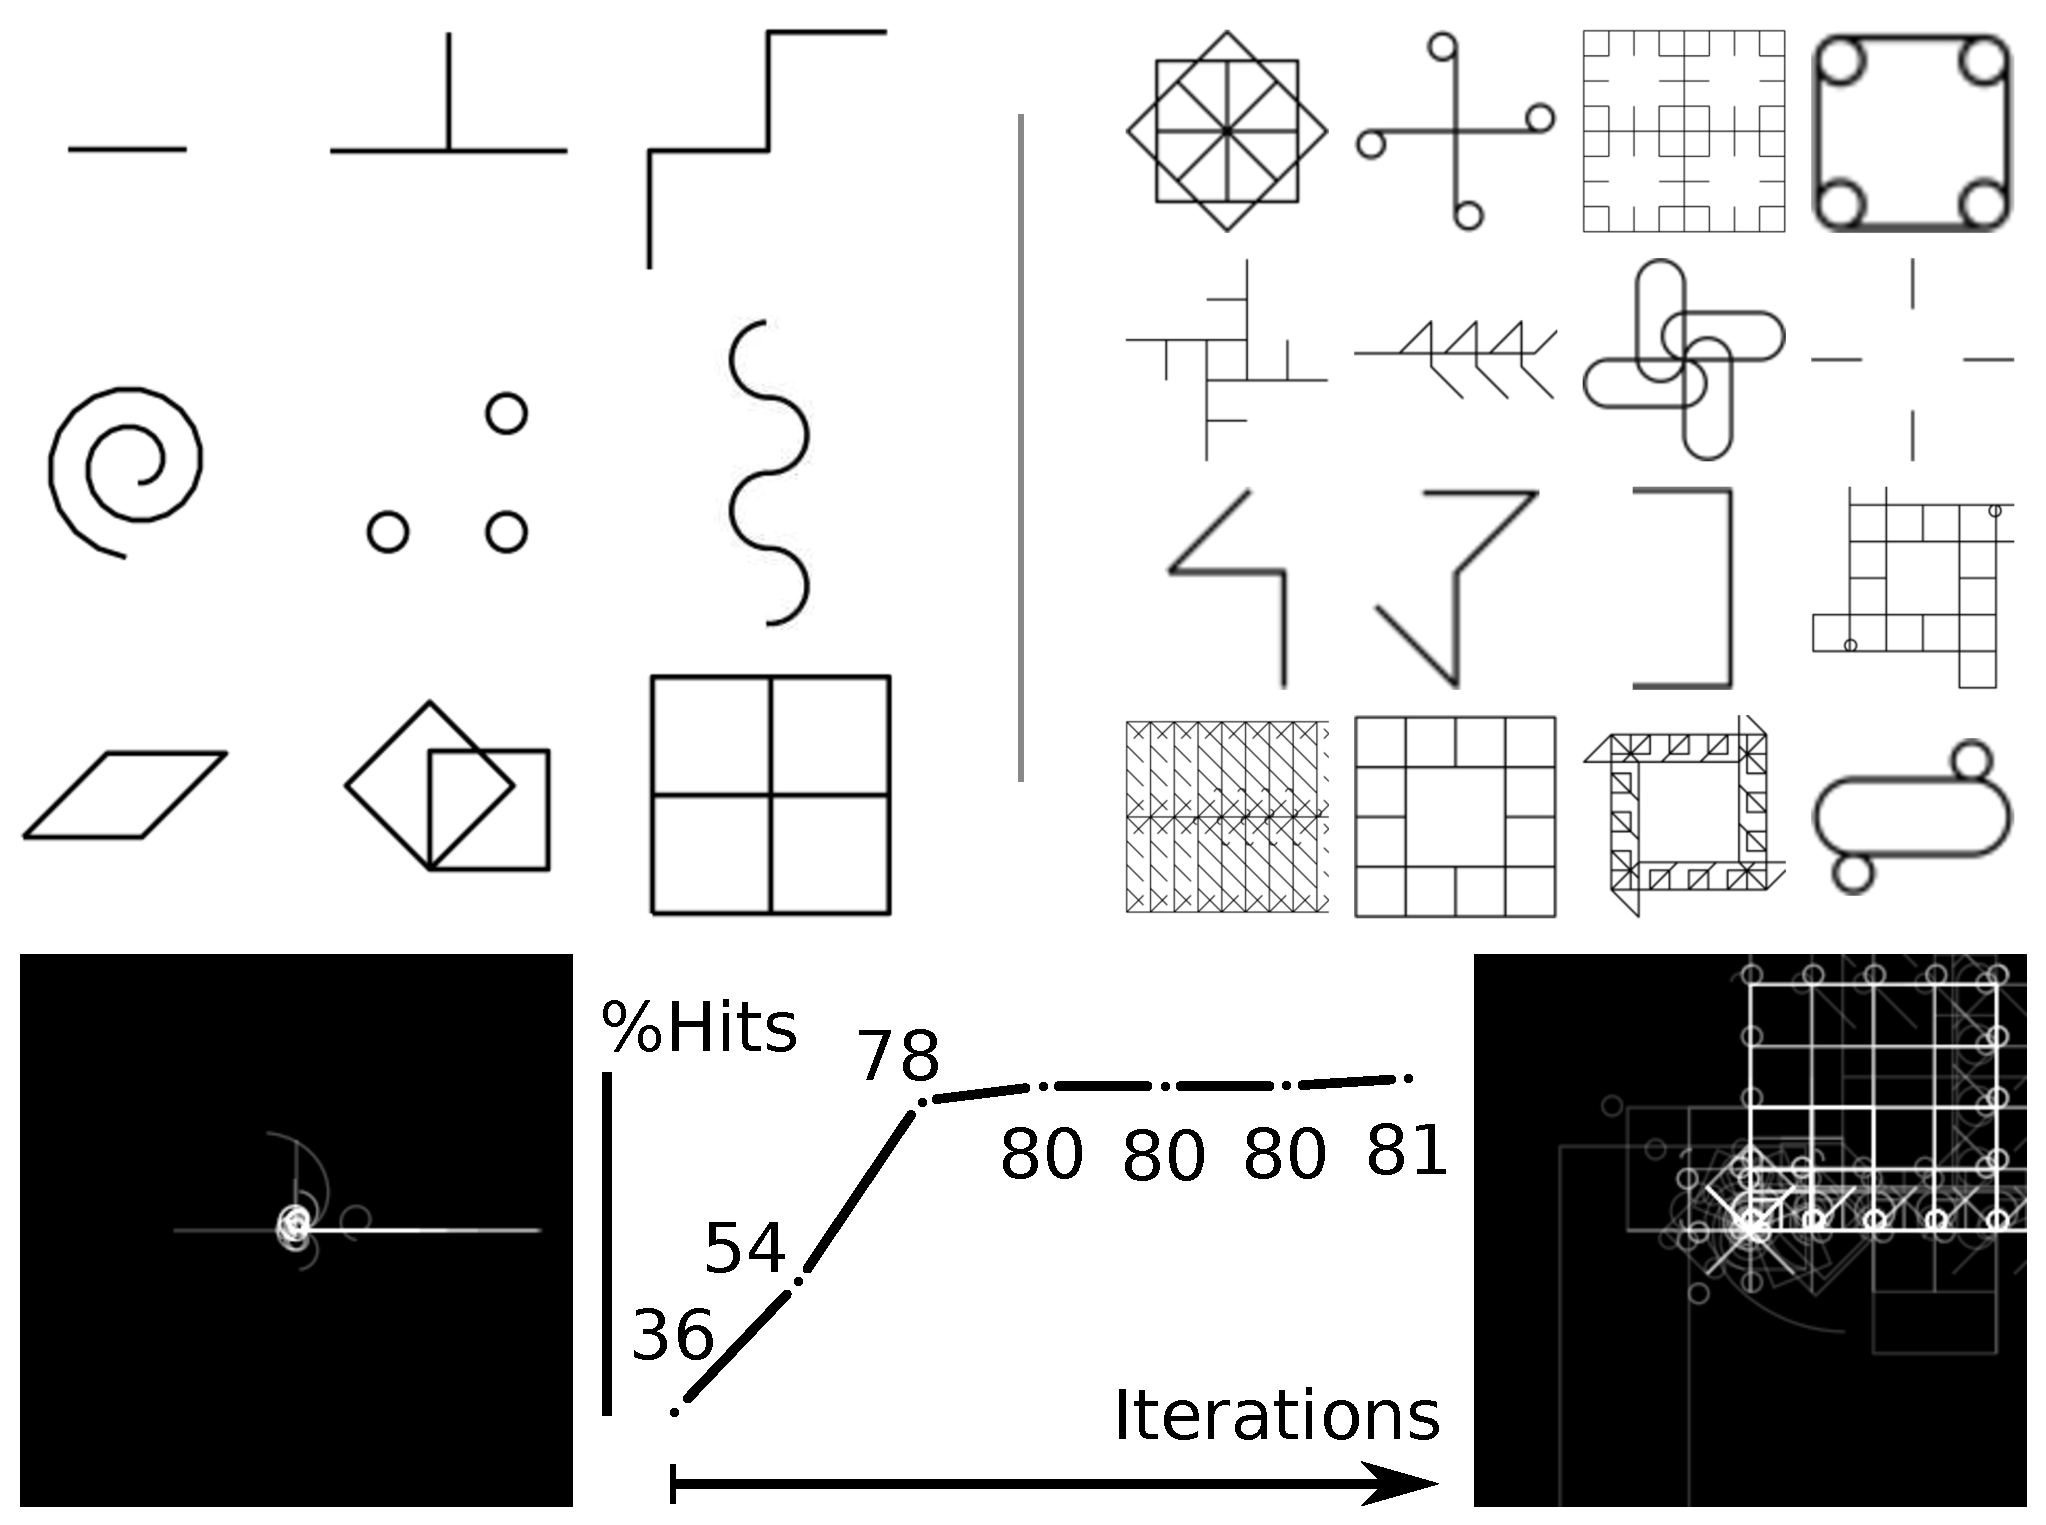
\includegraphics[width = 0.4\textwidth]{figures/geomCompiled.eps} 
  \end{center}
  \caption{
  Future: dreams.
  Top left: hand crafted traning targets. Top right: examples of
  discovered compiled new programs. Bottom: compiled programm across iterations
  to highlight structure emergence.
  }\label{geomCompiled} 
\end{wrapfigure}

We contribute an algorithm, \systemEnding, that learns to program by bootstrapping a DSL with new
domain-specific primitives that the algorithm itself discovers,
together with a neural recognition model that learns how to
efficiently deploy the DSL on new tasks. We believe this integration
of top-down symbolic representations and bottom-up neural networks --
both of them learned -- could help make program induction systems more
generally useful for AI. Many directions remain open. Two immediate
goals 
are to integrate more sophisticated neural recognition
models~\cite{devlin2017robustfill} and program
synthesizers~\cite{solar2008program}, which may improve performance in
some domains over the generic methods used here.
Another direction is to
explore DSL meta-learning: Can we find a \emph{single} universal
primitive set that could effectively bootstrap DSLs for new domains,
including the four domains considered,  but also many others?

\bibliographystyle{unsrt}
{\small \bibliography{main}}
\end{document}
